\documentclass[11pt,a4paper]{article}
\usepackage[T1]{fontenc}
\usepackage[utf8]{inputenc}
\usepackage[margin=19mm,headheight=14pt]{geometry}
\usepackage{lmodern,amsmath,amssymb,booktabs,xcolor,listings,enumitem,fancyhdr,graphicx}
\usepackage{placeins}
\usepackage[colorlinks=true,linkcolor=blue!50!black,urlcolor=blue!50!black]{hyperref}
\setlength{\parindent}{0pt}
\setlength{\parskip}{5pt}
\setlist[itemize]{leftmargin=*,topsep=3pt,itemsep=2pt,parsep=0pt}
\setlist[enumerate]{leftmargin=*,topsep=3pt,itemsep=2pt,parsep=0pt}
\pagestyle{fancy}
\fancyhf{}
\fancyhead[L]{Sampling}
\fancyhead[R]{Teacher's guide}
\fancyfoot[C]{\thepage}
\definecolor{codebg}{RGB}{246,247,249}
\lstset{language=Python,basicstyle=\ttfamily\footnotesize,
  keywordstyle=\color{blue!55!black},commentstyle=\color{black!60},
  stringstyle=\color{green!35!black},backgroundcolor=\color{codebg},
  frame=single,rulecolor=\color{black!15},framesep=5pt,
  showstringspaces=false,keepspaces=true,columns=fullflexible,
  breaklines=true,aboveskip=6pt,belowskip=6pt}
\newcommand{\E}{\mathbb E}
\newcommand{\Var}{\operatorname{Var}}
\newcommand{\Cov}{\operatorname{Cov}}
\newcommand{\ind}{\mathbf 1}
\newcommand{\Normal}{\mathcal N}
\newcommand{\MCSE}{\operatorname{MCSE}}
\newcommand{\ESS}{\operatorname{ESS}}
\begin{document}
\begin{center}
  {\LARGE\bfseries Sampling: from independent draws to Markov chains}\\[6pt]
  {\large Teacher's guide and worked solutions}\\[3pt]
  Bayesian machine learning \textbar\ Skoltech
\end{center}

Sampling methods turn integrals into averages. Their outputs can look similar
while having different mathematical meanings: rejection sampling gives
independent target draws, importance sampling gives weighted proposal draws,
and Markov chain Monte Carlo gives dependent states with a chosen stationary
distribution. This guide develops the theory needed to implement and compare
these methods, then gives solutions to three main tasks and an appendix task.

The implementations use NumPy and SciPy. A single parameter and a tractable
posterior make it possible to check every method against exact integrals.
The same principles extend to models whose posterior normalizer and moments
are unavailable. The numerical experiments should be read as controlled
examples of the theory, with attention to the distinction between a correct
algorithm and a favorable random realization.

\section{Monte Carlo integration}
\subsection{Why Bayesian inference leads to expectations}
Let $D$ denote observed data and let $\theta$ be a model parameter. Bayes' rule is
\[
 p(\theta\mid D)=\frac{p(D\mid\theta)p(\theta)}{p(D)},\qquad
 p(D)=\int p(D\mid\theta)p(\theta)\,d\theta.
\]
The denominator makes the posterior integrate to one. Evaluating the numerator
at a given parameter is often much easier than integrating it over the whole
parameter space.

For a future observation $y_*$ with input $x_*$, conditional independence of
the future response and training data given the parameter gives
\[
 p(y_*\mid x_*,D)
 =\int p(y_*\mid x_*,\theta)p(\theta\mid D)\,d\theta
 =\E_{p(\theta\mid D)}[p(y_*\mid x_*,\theta)].
\]
The parameter is integrated out. It should therefore not remain among the
conditioning arguments on the left. If posterior draws are available, we
average the conditional probabilities evaluated at those draws. Posterior
means, event probabilities, and expected losses are instances of the same
problem:
\[
 I=\int f(x)\pi(x)\,dx=\E_\pi[f(X)].
\]
An event probability uses an indicator, $f(x)=\ind\{x\in A\}$. A predictive
probability uses a conditional probability as $f$. The distribution $\pi$ and
function $f$ play separate roles, and the difficulty of estimating $I$ depends
on both.

\subsection{Unbiasedness, consistency, and variance}
Suppose $X_1,\ldots,X_N$ are independent and identically distributed with density
$\pi$. The Monte Carlo estimator is
\[
 \widehat I_N=\frac1N\sum_{i=1}^N f(X_i).
\]
If $\E_\pi|f(X)|<\infty$, linearity of expectation gives
\[
 \E[\widehat I_N]
 =\frac1N\sum_{i=1}^N\E[f(X_i)]=I.
\]
Thus it is unbiased at each sample size. Unbiasedness is an average over
repeated realizations of the whole experiment. It does not say that a
particular estimate is exact, or that its error decreases monotonically as
more samples are added.

The strong law of large numbers gives
\[
 \widehat I_N\longrightarrow I\quad\text{almost surely}
\]
under the iid and integrability assumptions above. This is a consistency
statement. When $\sigma_f^2=\Var_\pi f(X)<\infty$, independence also gives an
explicit finite-sample variance:
\begin{align*}
 \Var(\widehat I_N)
 &=\frac1{N^2}\sum_{i=1}^N\sum_{j=1}^N
       \Cov(f(X_i),f(X_j))\\
 &=\frac1{N^2}\sum_{i=1}^N\sigma_f^2
 =\frac{\sigma_f^2}{N}.
\end{align*}
The off-diagonal covariances vanish because the draws are independent.
Chebyshev's inequality provides a direct finite-variance route to convergence
in probability:
\[
 \Pr(|\widehat I_N-I|>\varepsilon)
 \le\frac{\sigma_f^2}{N\varepsilon^2}\longrightarrow0.
\]
The bound is often conservative, but it makes the source of the
$N^{-1/2}$ error scale explicit.

The root mean squared error is
$\operatorname{RMSE}(\widehat I_N)=\sqrt{\E[(\widehat I_N-I)^2]}$.
For any square-integrable estimator, expanding around its expectation gives
\[
 \E[(\widehat I_N-I)^2]
 =\Var(\widehat I_N)+(\E\widehat I_N-I)^2.
\]
For iid Monte Carlo the bias term vanishes, so RMSE is $\sigma_f/\sqrt N$.
For a biased estimator such as self-normalized importance sampling, both terms
matter. An empirical RMSE from independent replications estimates their
combined effect.

\subsection{The central limit theorem and Monte Carlo standard error}
For iid draws with $0<\sigma_f^2<\infty$, the central limit theorem states
\[
 \frac{\sqrt N(\widehat I_N-I)}{\sigma_f}
 \ \xrightarrow{d}\ \Normal(0,1).
\]
It is a limiting statement about the estimator's error distribution, not an
assertion that a finite-sample average is exactly Gaussian. Replacing
$\sigma_f^2$ with the sample variance gives
\[
 s_f^2=\frac1{N-1}\sum_i(f(X_i)-\widehat I_N)^2,\qquad
 \widehat{\MCSE}(\widehat I_N)=\frac{s_f}{\sqrt N}.
\]
An interval such as $\widehat I_N\pm1.96\,\widehat{\MCSE}$ has approximate
repeated-experiment coverage when the normal approximation is adequate.
For rare events, too few observed events can make this approximation poor.
Observing zero events does not establish that the true probability is zero.

The standard deviation $\sigma_f$ describes variation in the integrand under
the target. MCSE describes variation in the numerical estimate of its
expectation. For $f(\theta)=\theta$, a posterior interval describes uncertainty
about the parameter under the model; an MCSE interval describes numerical
error in computing its posterior mean. More draws can shrink the second while
leaving the first unchanged.

\begin{figure}[htbp]
\centering
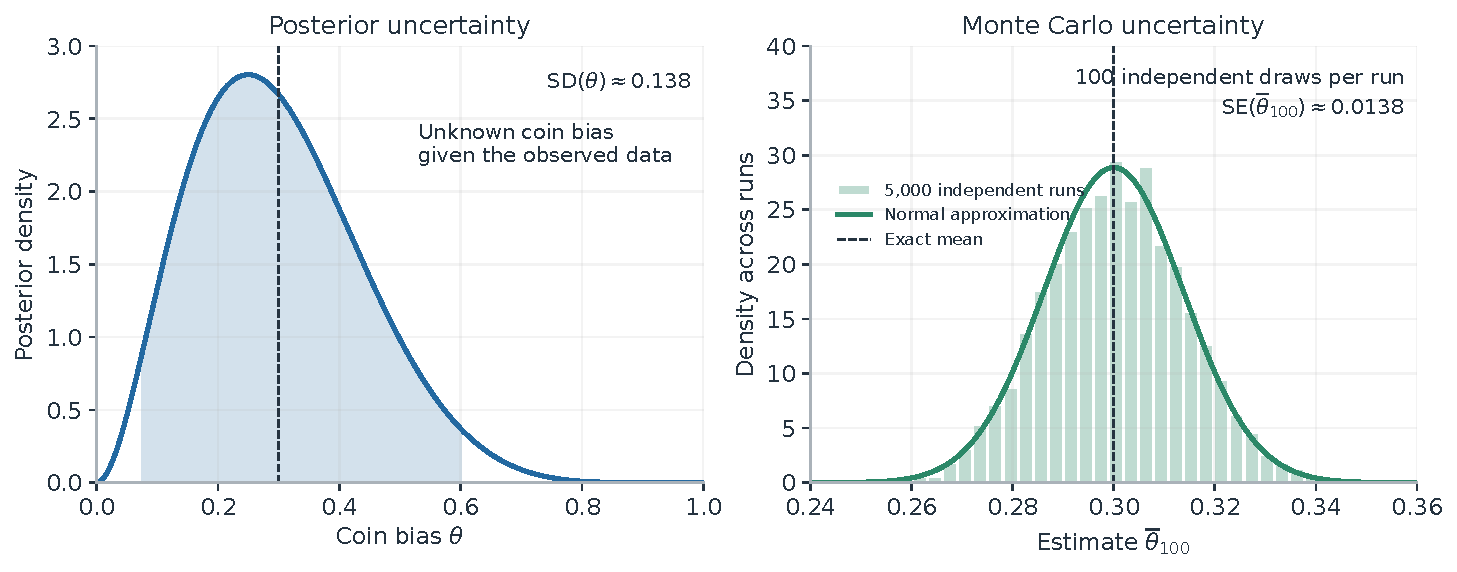
\includegraphics[width=\linewidth]{assets/monte_carlo_uncertainty.pdf}
\caption{Posterior draws from $\operatorname{Beta}(3,7)$ and estimates of its
mean from 100 independent draws describe different random quantities.
The panels use different horizontal scales. Increasing the draw count can
concentrate the estimates while leaving the posterior unchanged.}
\end{figure}

The exponent in the iid error rate does not explicitly depend on dimension.
The variance constant $\Var_\pi f(X)$ can nevertheless grow with dimension,
and obtaining useful draws can become much harder. Four times as many
independent draws approximately halves MCSE. This concerns the distribution
of error; one run's error can increase after adding observations.

\subsection{Inverse CDF sampling}
Inverse transform sampling converts uniform randomness into draws from a
specified distribution. Suppose first that a continuous CDF $F$ is strictly
increasing on its support. For $U\sim U(0,1)$, let $X=F^{-1}(U)$. Then
\[
 \Pr(X\le x)=\Pr(F^{-1}(U)\le x)=\Pr(U\le F(x))=F(x).
\]
Hence $X$ has CDF $F$. For an arbitrary CDF, the generalized inverse
$F^{-1}(u)=\inf\{x:F(x)\ge u\}$ gives the corresponding construction even when
an ordinary inverse does not exist. The claim that $F(X)$ is uniform, in
contrast, needs continuity; atoms require care.

For an exponential distribution with rate $\lambda=2$,
\[
 F(x)=1-e^{-2x},\quad x\ge0,\qquad
 X=-\frac12\log(1-U),\qquad
 \E X=\frac12,\quad\Var X=\frac14.
\]
The rate is the reciprocal of the scale. The stable numerical expression is
\texttt{-np.log1p(-u) / 2.0}, which avoids loss of relative accuracy when
computing $\log(1-u)$ for small $u$.

\begin{figure}[htbp]
\centering
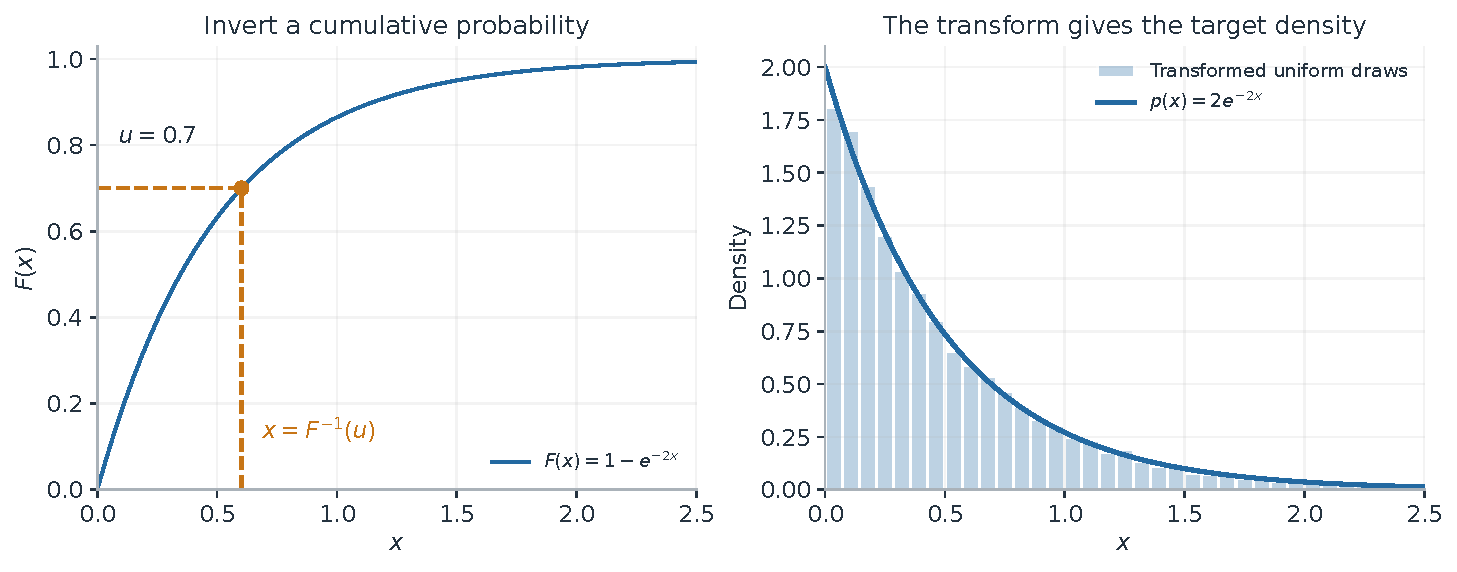
\includegraphics[width=\linewidth]{assets/inverse_cdf.pdf}
\caption{Inverse transform sampling reads a uniform height on the CDF axis
and maps it to a location on the sample axis. The exponential distribution has
an analytic inverse, so no rejection or Markov chain is needed.}
\end{figure}

This example separates a sampling rule from the Monte Carlo estimator applied
to its output. Once draws have the correct distribution, the same sample can
estimate many expectations. In more complex models the inverse CDF is
unavailable, motivating the three tasks below.

\FloatBarrier
\section{A posterior with an exact reference}
\subsection{The beta--Bernoulli model}
Let $\theta\in(0,1)$ denote a coin's probability of heads. Conditional on
$\theta$, the observed tosses are independent Bernoulli variables. If there are
$h$ heads and $t$ tails in an observed sequence, its likelihood is
\[
 p(D\mid\theta)=\theta^h(1-\theta)^t.
\]
If the observation is instead an unordered head count, a binomial coefficient
multiplies this expression. That coefficient is independent of $\theta$, so
the posterior kernel is unchanged.

For positive shape parameters $a_0,b_0$, the beta density is
\[
 p(\theta)=\frac{\theta^{a_0-1}(1-\theta)^{b_0-1}}{B(a_0,b_0)},\qquad
 B(a,b)=\int_0^1u^{a-1}(1-u)^{b-1}\,du.
\]
Multiplication by the likelihood adds observed counts to the exponents:
\[
 p(\theta\mid D)\propto
 \theta^{a_0+h-1}(1-\theta)^{b_0+t-1}.
\]
A beta prior is therefore conjugate to Bernoulli observations, with posterior
$\operatorname{Beta}(a_0+h,b_0+t)$.

Here $a_0=b_0=2$, $h=1$, and $t=5$. We choose the unnormalized kernel
\[
 \widetilde\pi(\theta)=\theta^2(1-\theta)^6\ind\{0<\theta<1\},\qquad
 \pi(\theta)=\frac{\widetilde\pi(\theta)}Z
 =\operatorname{Beta}(\theta;3,7).
\]
The constant $Z$ normalizes this chosen kernel. Since constants from the prior
density and likelihood may have been omitted, $Z$ is not automatically the
model's marginal likelihood. For integer beta parameters,
\[
 Z=B(3,7)=\frac{\Gamma(3)\Gamma(7)}{\Gamma(10)}
 =\frac{2!\,6!}{9!}=\frac1{252}.
\]
The tasks operate on $\widetilde\pi$ without calling a direct
$\operatorname{Beta}(3,7)$ sampler. The normalized density serves as a reference
for auditing the algorithms.

\subsection{Exact moments and a posterior event probability}
For $\Theta\sim\operatorname{Beta}(a,b)$ and nonnegative integer $k$, direct integration gives
\[
 \E\Theta^k=\frac{B(a+k,b)}{B(a,b)}.
\]
Using $B(a+1,b)=aB(a,b)/(a+b)$ yields
\[
 \E\Theta=\frac a{a+b},\qquad
 \E\Theta^2=\frac{a(a+1)}{(a+b)(a+b+1)},\qquad
 \Var\Theta=\frac{ab}{(a+b)^2(a+b+1)}.
\]
Consequently, the two shared estimands and posterior variance are
\[
 I_1=\E_\pi\Theta=0.3,\qquad
 \Var_\pi\Theta=\frac{21}{1100}\simeq0.0190909,\qquad
 I_2=\Pr_\pi(\Theta>1/2)=\frac{23}{256}=0.08984375.
\]
The mean is also the posterior predictive probability of a head on the next
toss because $\Pr(H_{\rm next}\mid\Theta)=\Theta$.

The tail reference can be derived without simulation. An antiderivative of
$\theta^2(1-\theta)^6$ is
\[
 A(\theta)=\frac{\theta^3}{3}-\frac{6\theta^4}{4}
 +\frac{15\theta^5}{5}-\frac{20\theta^6}{6}
 +\frac{15\theta^7}{7}-\frac{6\theta^8}{8}+\frac{\theta^9}{9}.
\]
Therefore $I_2=252[A(1)-A(1/2)]=23/256$. Equivalently, the integer-shape
beta--binomial identity gives
$I_2=2^{-9}\sum_{k=0}^{2}\binom9k=(1+9+36)/512$.
The event probability is an expectation of
$f(\theta)=\ind\{\theta>1/2\}$, so it needs no new sampling rule.

\subsection{Evaluating the target in log space}
Inside the support,
$\log\widetilde\pi(\theta)=2\log\theta+6\log(1-\theta)$.
Outside it, the log kernel is $-\infty$. The helper below preserves valid
interior arguments while avoiding logarithms of invalid ones:
\begin{lstlisting}
import numpy as np
from scipy.special import logsumexp
from scipy.stats import norm

def log_target(theta):
    theta = np.asarray(theta, dtype=float)
    inside = (theta > 0.0) & (theta < 1.0)
    safe = np.where(inside, theta, 0.5)
    value = 2*np.log(safe) + 6*np.log1p(-safe)
    return np.where(inside, value, -np.inf)
\end{lstlisting}
Replacing out-of-support arguments temporarily only prevents invalid
arithmetic; the final result still assigns them zero density. Clipping valid
interior arguments to an arbitrary tolerance would change the declared target
near its boundaries and is unnecessary.

\section{Task 1: rejection sampling}
\subsection{The envelope and the augmented joint law}
Suppose $q$ is a normalized density from which independent proposals can be
drawn, and a finite constant $M$ satisfies
\[
 0\le\widetilde\pi(x)\le Mq(x)\quad\text{for every }x.
\]
This requires $q$ to cover the target support and to be large enough relative
to the kernel everywhere. A proposal with lighter tails than the target may
admit no finite envelope even if it resembles the target near its mode.

Draw $Y\sim q$ and $U\sim U(0,1)$ independently, and retain $Y$ on the event
\[
 A=\left\{U<\frac{\widetilde\pi(Y)}{Mq(Y)}\right\}.
\]
The joint density of $(Y,U)$ is $q(y)$ on $0<u<1$. Integrating over the
accepted vertical segment gives
\[
 p(Y\in dy,A)=q(y)\frac{\widetilde\pi(y)}{Mq(y)}\,dy
 =\frac{\widetilde\pi(y)}M\,dy.
\]
Integrating once more yields the acceptance probability
\[
 a=\Pr(A)=\frac1M\int\widetilde\pi(y)\,dy=\frac ZM.
\]
Dividing the accepted joint mass by $a$ shows that
\[
 p(y\mid A)=\frac{\widetilde\pi(y)/M}{Z/M}=\pi(y).
\]
An alternative geometric construction draws a height
$T\mid Y=y\sim U(0,Mq(y))$. Its joint density with $Y$ is $1/M$ under the
envelope. Conditioning on $0<T<\widetilde\pi(Y)$ gives the target marginal.
The area under the kernel divided by the area under the envelope is $Z/M$.

\begin{figure}[htbp]
\centering
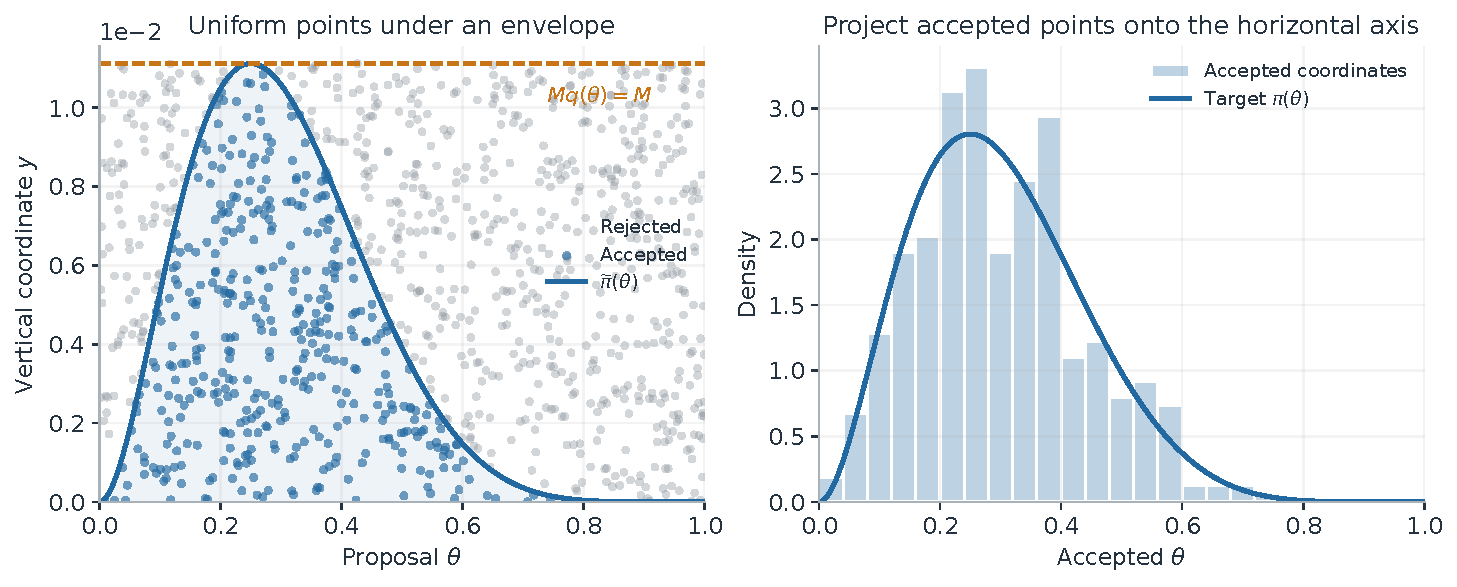
\includegraphics[width=\linewidth]{assets/rejection_geometry.pdf}
\caption{Rejection sampling augments each proposal with an independent height.
Keeping points below the target kernel gives a horizontal marginal proportional
to that kernel. The unused part of the envelope determines rejection cost.}
\end{figure}

The acceptance formula $1/M$ applies only when the target in the envelope
is normalized. Here $M$ bounds an unnormalized kernel and can be less than one.
Multiplying the kernel and envelope by the same positive constant changes
neither acceptance decisions nor the conditional law.

\subsection{A uniform envelope for the coin posterior}
Use $q(\theta)=1$ on $(0,1)$. Maximizing the log kernel gives
\[
 \frac{d}{d\theta}\log\widetilde\pi(\theta)
 =\frac2\theta-\frac6{1-\theta}=0
 \quad\Longrightarrow\quad\theta_{\rm mode}=\frac14.
\]
Its second derivative is
$-2/\theta^2-6/(1-\theta)^2<0$, so this is the unique interior maximum.
The kernel tends to zero at both boundaries. A tight envelope is therefore
\[
 M=\left(\frac14\right)^2\left(\frac34\right)^6
 =\frac{729}{65536}\simeq0.01112366,
 \qquad a=\frac ZM\simeq0.35674004.
\]
An underestimated envelope makes some nominal acceptance probabilities exceed
one. Clipping them to one does not repair the derivation: the accepted density
is then proportional to $\min\{\widetilde\pi,Mq\}$ rather than the target
kernel. A larger valid envelope preserves correctness and reduces efficiency.

\subsection{Implementation and output contract}
The function \texttt{rejection\_sample} takes \texttt{n\_proposals} and
\texttt{rng}. It returns accepted values and a Boolean mask with one entry per proposal. The proposal
budget is fixed at 20,000; the retained count is random. Candidate uniforms
and acceptance uniforms must be independent.
\begin{lstlisting}
def rejection_sample(n_proposals, rng):
    candidates = rng.uniform(0.0, 1.0, size=n_proposals)
    uniforms = rng.uniform(0.0, 1.0, size=n_proposals)
    envelope = (1.0 / 4.0)**2 * (3.0 / 4.0)**6
    kernel = candidates**2 * (1.0 - candidates)**6
    mask = uniforms < kernel / envelope
    return candidates[mask], mask
\end{lstlisting}
For independent proposal--uniform pairs, accepted locations are independent
target draws. Conditional on the accepted count $K=k>0$ under a fixed proposal
budget, retained locations have the iid target law. Their sample-based
Monte Carlo standard error therefore uses $k$:
\begin{lstlisting}
rng = np.random.default_rng(11)
accepted, mask = rejection_sample(20_000, rng)
mean_estimate = accepted.mean()
mean_se = accepted.std(ddof=1) / np.sqrt(len(accepted))
tail_values = (accepted > 0.5).astype(float)
tail_estimate = tail_values.mean()
tail_se = tail_values.std(ddof=1) / np.sqrt(len(accepted))
acceptance_estimate = mask.mean()
\end{lstlisting}
At least two accepted values are needed for a sample variance with
\texttt{ddof=1}. A general implementation should report insufficient samples
when that condition fails.

\subsection{Model answers and useful hints}
The count $K$ is binomial with mean $20{,}000a\simeq7{,}135$ and standard
deviation $\sqrt{20{,}000a(1-a)}\simeq67.7$. Its empirical acceptance rate
has standard deviation about $0.00339$. For a retained count near its mean,
the posterior mean's theoretical MCSE is approximately $0.00164$, while the
tail estimate's is approximately $0.00339$. These are error scales, not fixed
outputs or guarantees for a particular random seed.

A useful first hint is to construct two arrays of the same length. The next
hint is to evaluate the kernel at all candidates and divide by the envelope.
The final step is a Boolean comparison followed by \texttt{candidates[mask]}.
Returning indices instead of a mask changes the interface.

The posterior standard deviation is approximately $0.13817$, much larger
than the MCSE of its estimated mean. A density histogram of accepted values
estimates the posterior; a histogram of all candidates estimates the proposal.
Keeping rejected candidates would mix two different sampling laws.

The method needs about $1/a\simeq2.8$ proposals per retained draw on average.
This describes proposal cost, rather than a complete comparison with other
methods: evaluating a proposal, its density, and the target can have different
costs in different models.

\section{Task 2: self-normalized importance sampling}
\subsection{Changing the sampling distribution}
Importance sampling changes the distribution generating locations and
compensates with a density ratio. Suppose the normalized target $\pi$ is
known, $Y_i\sim q$ independently, and $q(x)>0$ wherever
$|f(x)|\pi(x)>0$. Then
\[
 I=\int f(x)\pi(x)\,dx
   =\int f(x)\frac{\pi(x)}{q(x)}q(x)\,dx
   =\E_q\left[\frac{\pi(Y)}{q(Y)}f(Y)\right].
\]
The ordinary importance estimator is
\[
 \widehat I_{\rm IS}=\frac1N\sum_{i=1}^N\frac{\pi(Y_i)}{q(Y_i)}f(Y_i).
\]
If the absolute expectation exists, it is unbiased. If its second moment is
finite, its variance is
\[
 \Var(\widehat I_{\rm IS})=
 \frac1N\left[\int\frac{\pi(x)^2f(x)^2}{q(x)}\,dx-I^2\right].
\]
Small $q$ where $|f|\pi$ is appreciable can make this variance very large or
infinite. Sampling from another distribution is useful only when its
importance correction remains manageable.

For several estimands, requiring $q>0$ on the whole target support is a
convenient condition. It is essential for the self-normalized construction
below, whose denominator must estimate the entire target mass.

\subsection{The ratio estimator when the normalizer is unknown}
Let $\pi=\widetilde\pi/Z$ and define
$w(x)=\widetilde\pi(x)/q(x)$. Coverage of the target support gives
\[
 \E_q[w(Y)]=Z,\qquad \E_q[w(Y)f(Y)]=ZI.
\]
Estimate both expectations from the same draws:
\[
 \widehat I_{\rm SNIS}
 =\frac{N^{-1}\sum_iw_i f(Y_i)}{N^{-1}\sum_iw_i}
 =\sum_i\bar w_i f(Y_i),\qquad
 \bar w_i=\frac{w_i}{\sum_jw_j}.
\]
The unknown $Z$ cancels. The locations still have law $q$: weighting changes
the estimator, not their sampling distribution. Resampling from the weighted
empirical distribution is a separate operation and is unnecessary for these
expectations.

The expectation of a ratio is generally not the ratio of expectations.
SNIS is therefore generally biased at finite $N$. A constant integrand is a
special case with zero bias, not a proof of general unbiasedness. With
$0<Z<\infty$, coverage, and $\E_\pi|f|<\infty$, the laws of large numbers for
numerator and denominator imply almost sure consistency wherever the ratio
is defined. A positive weight sum is required; proposals entirely outside
target support cannot produce an estimate.

\subsection{Asymptotic variance and a plug-in MCSE}
The centered ratio has the exact representation
\[
 \sqrt N(\widehat I_{\rm SNIS}-I)
 =\frac{N^{-1/2}\sum_iw_i(f(Y_i)-I)}{N^{-1}\sum_iw_i}.
\]
The numerator summands have mean zero. If
$\E_q[w^2(f-I)^2]<\infty$, their iid central limit theorem and the
denominator's law of large numbers give
\[
 \sqrt N(\widehat I_{\rm SNIS}-I)
 \ \xrightarrow{d}\ \Normal(0,\sigma_{\rm SNIS,f}^2),\qquad
 \sigma_{\rm SNIS,f}^2=\frac{\E_q[w^2(f-I)^2]}{Z^2}.
\]
The variance depends on $f$. A proposal that estimates the mean well need
not be best for an event probability.

Replacing the unknown terms by their sample counterparts yields
\[
 \widehat{\MCSE}_{\rm SNIS}
 =\sqrt{\sum_i\bar w_i^2(f(Y_i)-\widehat I_{\rm SNIS})^2}.
\]
The squared expression is the plug-in estimate of
$\sigma_{\rm SNIS,f}^2/N$. It is a large-sample estimate under iid covered
proposal sampling and a finite weighted second moment. It is not an unbiased
finite-sample variance estimator or a remedy for an unvisited important region.
Compute it separately for the mean and tail indicator.

The ratio estimator and importance-sampling error analysis are developed in
Owen's treatment \cite{owen}. The practical questions are whether the proposal
covers the target and whether the relevant weighted moments are finite.

\subsection{Stable normalized weights and weight ESS}
Raw importance weights can overflow or underflow. Writing
$\ell_i=\log w_i$ and $a=\max_i\ell_i$ gives
\[
 v_i=e^{\ell_i-a},\qquad \bar w_i=\frac{v_i}{\sum_jv_j}.
\]
The common factor $e^{-a}$ cancels. Equivalently,
$\bar w_i=\exp(\ell_i-\operatorname{logsumexp}(\ell))$.
Adding a common finite constant to all log weights leaves the normalized
weights, estimates, and weight ESS unchanged.

The weight concentration diagnostic is
\[
 \ESS_w=\frac1{\sum_i\bar w_i^2}
 =\frac{(\sum_iw_i)^2}{\sum_iw_i^2}.
\]
Because $\sum_i\bar w_i=1$, Cauchy--Schwarz gives
$1\le N\sum_i\bar w_i^2$, so $\ESS_w\le N$. Nonnegativity implies
$\sum_i\bar w_i^2\le(\sum_i\bar w_i)^2=1$, giving $\ESS_w\ge1$.
Equal weights achieve $N$; concentration on one point gives one.

If $\E_qw^2<\infty$, a law of large numbers gives
\[
 \frac{\ESS_w}{N}
 =\frac{(N^{-1}\sum_iw_i)^2}{N^{-1}\sum_iw_i^2}
 \longrightarrow\frac{Z^2}{\E_qw^2}
 =\frac1{1+\Var_q(w)/Z^2}.
\]
Thus weight ESS measures weight dispersion. It is not an exact equivalent
count of target draws for every integrand: its formula contains no $f$, while
the SNIS asymptotic variance does. It also differs from the autocorrelation
MCMC ESS derived later.

\begin{figure}[htbp]
\centering
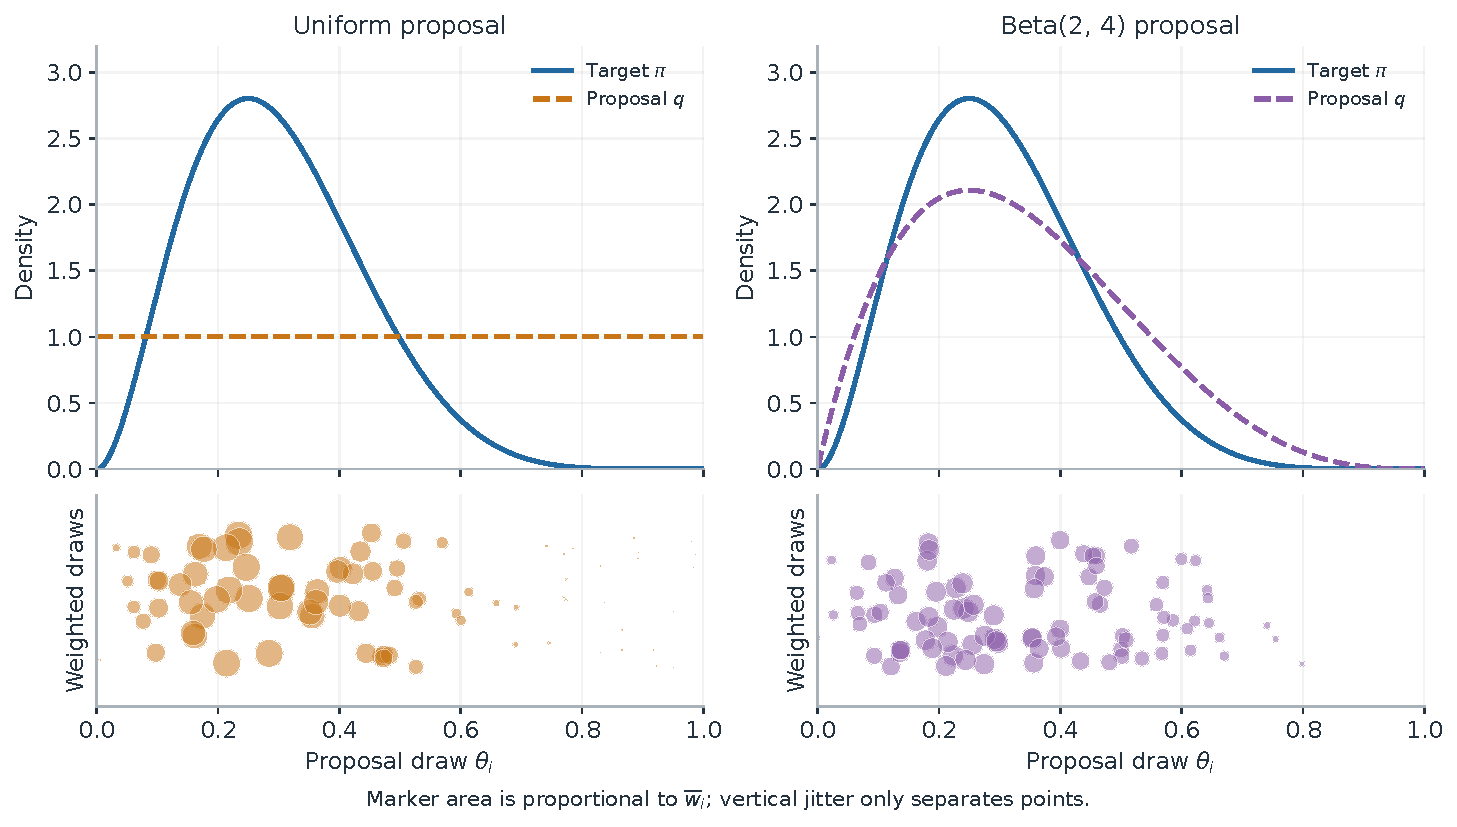
\includegraphics[width=\linewidth]{assets/importance_weights.pdf}
\caption{Importance sampling retains proposal locations and changes their
contributions to an estimate. Coverage and weight concentration both matter;
a weighted empirical distribution differs from an unweighted sample drawn
directly from the target.}
\end{figure}

\subsection{Implementation and the proposal comparison}
The function \texttt{snis} takes matching one-dimensional arrays of log weights
and finite values. At least one log weight is finite; others may be
$-\infty$ to represent zero weight. NaN and positive infinity are excluded.
It returns the estimate, normalized weights, and scalar weight ESS.
\begin{lstlisting}
def snis(log_weights, values):
    log_weights = np.asarray(log_weights, dtype=float)
    values = np.asarray(values, dtype=float)
    maximum = np.max(log_weights)
    weights = np.exp(log_weights - maximum)
    normalized_weights = weights / weights.sum()
    estimate = np.sum(normalized_weights * values)
    ess = 1.0 / np.sum(normalized_weights**2)
    return estimate, normalized_weights, ess
\end{lstlisting}
The returned weights also support weighted plots and the plug-in MCSE:
\begin{lstlisting}
estimate, normalized_weights, ess = snis(log_weights, values)
mcse = np.sqrt(np.sum(normalized_weights**2 * (values - estimate)**2))
\end{lstlisting}
Reuse locations and weights for both quantities. Use $x$ as the values for
the mean and the indicator $\ind\{x>0.5\}$ for the tail. An unweighted proposal mean
estimates an expectation under $q$. An average of unnormalized
\texttt{weights * values} estimates $ZI$ and cannot replace the ratio when
$Z$ is unknown.

The comparison uses $q_U=U(0,1)$ and $q_B=\operatorname{Beta}(2,4)$,
with 2,000 proposals each. Under the uniform proposal,
$w_U=\widetilde\pi$. Since $B(2,4)=1/20$,
\[
 q_B(\theta)=20\theta(1-\theta)^3,\qquad
 w_B(\theta)=\frac{\theta(1-\theta)^3}{20}.
\]
Both proposals cover $(0,1)$ and have finite relevant second moments. The
beta proposal concentrates more mass in the posterior's high-density region
and typically gives more balanced weights.

For these proposals,
\[
 \E_{q_U}w^2=B(5,13),\qquad
 \E_{q_B}w^2=\frac{B(4,10)}{20}.
\]
The limiting ESS fractions are approximately $0.487$ and $0.901$.
At 2,000 draws, weight ESS values around 975 and 1,800 are reasonable
scales, not requirements for every realization.

\subsection{Model answers, repeated estimates, and hints}
The repeated experiment uses 100 independent replications with 500 proposals
each. For estimates $\widehat I_r$, empirical bias and RMSE are
\[
 \widehat{\operatorname{bias}}=\frac1R\sum_r\widehat I_r-I,\qquad
 \widehat{\operatorname{RMSE}}=
 \sqrt{\frac1R\sum_r(\widehat I_r-I)^2}.
\]
The mean's asymptotic error scales at this proposal count are approximately
$0.0067$ for uniform proposals and $0.0055$ for beta proposals. For the tail,
they are closer: approximately $0.0108$ and $0.0101$. Finite replication
error can reverse small differences. A small empirical bias does not establish
finite-sample unbiasedness.

A useful sequence of hints is to normalize log weights, form a weighted sum,
then compute the squared-weight sum. Equal weights should give the arithmetic
mean and ESS $N$. A single nonzero weight gives its location's value and ESS
one. Adding 1000 to every log weight tests stability and invariance to a
target normalizer.

The explanation should distinguish increased weight ESS from a universal
accuracy claim. A proposal can miss an important region and still produce
apparently even weights among observed points. Neither large observed ESS
nor a narrow plug-in MCSE establishes adequate coverage from observations
alone. Both rely on proposal and moment assumptions.

\section{Task 3: random-walk Metropolis--Hastings}
\subsection{A Markov chain and its stationary law}
A Markov chain has conditional independence
\[
 p(x_{t+1}\mid x_0,\ldots,x_t)=p(x_{t+1}\mid x_t).
\]
A time-homogeneous kernel $K(x,A)$ gives the probability of moving from $x$
into a measurable set $A$, using the same rule at every iteration. A
distribution $\pi$ is stationary for $K$ if
\[
 \pi(A)=\int K(x,A)\pi(x)\,dx
\]
for every $A$. Starting a chain in $\pi$ preserves that marginal law after
each transition. Starting elsewhere need not produce that law immediately.

MCMC builds a usable kernel with the desired stationary distribution.
Stationarity is invariance; convergence from other starts also needs suitable
irreducibility, recurrence, and aperiodicity conditions. Even an ergodic chain
can mix too slowly for a practical run. Finite-run diagnostics assess
consequences of this difficulty without proving the absence of unseen problems.

\subsection{Acceptance and the full transition kernel}
From current state $x$ with positive target density, propose
$Y\sim q(\cdot\mid x)$ and accept with probability
\[
 \alpha(x,y)=\min\left\{1,
 \frac{\widetilde\pi(y)q(x\mid y)}
      {\widetilde\pi(x)q(y\mid x)}\right\}.
\]
A zero reverse proposal density or zero candidate target density gives
acceptance zero. The unknown target normalizer cancels in the ratio.

The transition includes a continuous move and a point mass at the current
state:
\[
 K(x,dy)=q(y\mid x)\alpha(x,y)\,dy+r(x)\delta_x(dy),\qquad
 r(x)=1-\int q(z\mid x)\alpha(x,z)\,dz.
\]
Here $\delta_x$ puts all mass at $x$. The continuous accepted-move density
usually integrates to less than one. The holding mass completes the transition
and is the mathematical reason repeated states must be stored.

The accepted flow satisfies
\begin{align*}
 \pi(x)q(y\mid x)\alpha(x,y)
 &=\min\{\pi(x)q(y\mid x),\pi(y)q(x\mid y)\}\\
 &=\pi(y)q(x\mid y)\alpha(y,x).
\end{align*}
The holding part lies on the diagonal $x=y$ and is symmetric too. Thus
$\pi(dx)K(x,dy)=\pi(dy)K(y,dx)$, the detailed balance identity.
Integrating over $x$ gives stationarity:
\[
 \int\pi(dx)K(x,A)
 =\int_A\pi(dy)\int K(y,dx)=\pi(A).
\]
Detailed balance is a sufficient construction of stationarity; it is not a
necessary property of every MCMC method.

\begin{figure}[htbp]
\centering
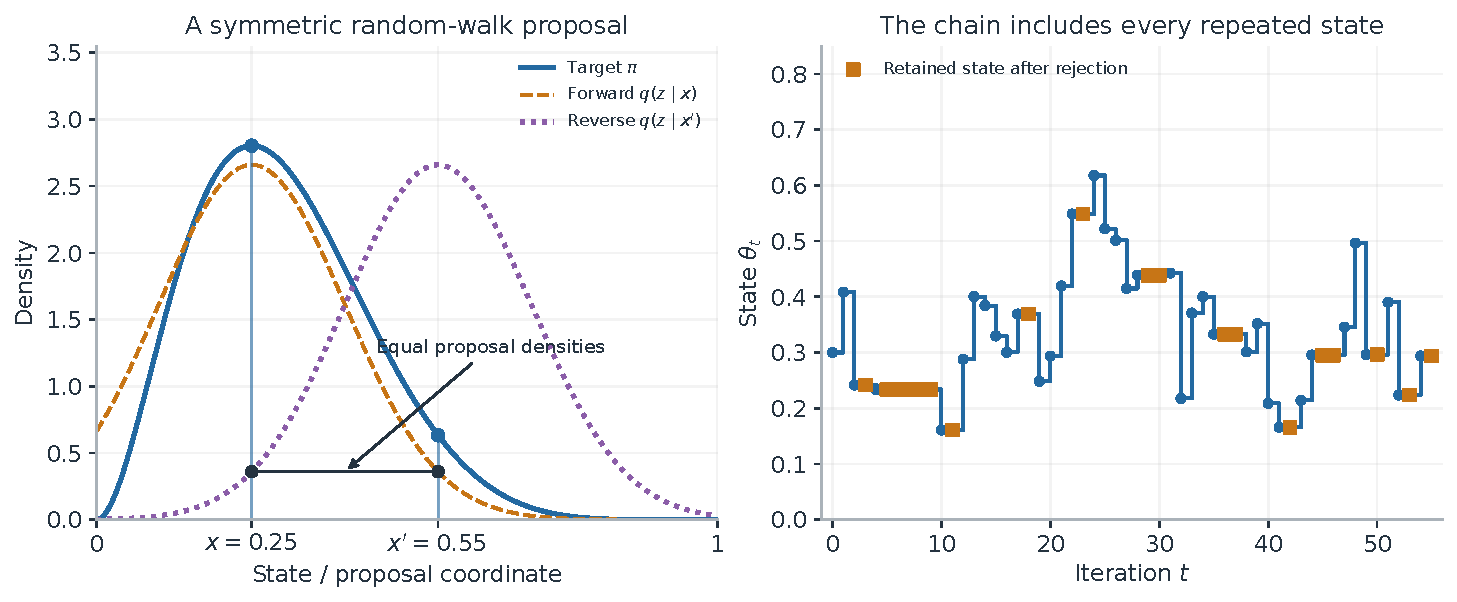
\includegraphics[width=\linewidth]{assets/metropolis_geometry.pdf}
\caption{A Metropolis step combines a proposal with an acceptance decision.
Rejection is a genuine holding probability. Small proposals can be accepted
frequently while moving slowly through the target.}
\end{figure}

\subsection{Symmetric Gaussian proposals and log-space decisions}
For the random walk
\[
 Y=x+s\varepsilon,\quad \varepsilon\sim\Normal(0,1),\qquad
 q(y\mid x)=\Normal(y;x,s^2),
\]
forward and reverse densities are equal. Therefore
\[
 \log\alpha(x,y)=\min\{0,
 \log\widetilde\pi(y)-\log\widetilde\pi(x)\}.
\]
Accepting when $\log U<\log\alpha$ avoids exponentiating a potentially
enormous density ratio. An out-of-support candidate has log target $-\infty$
and is rejected. Initial states must have finite log target.

The Gaussian proposal is sampled on its full support, and outside candidates
are rejected. Moving an outside candidate into the target interior changes the
accepted proposal kernel. In this example, mapping it exactly to an endpoint
and still assigning that endpoint log target $-\infty$ gives the same rejection
decision, but serves no purpose. Resampling until a candidate is inside instead
produces a truncated proposal whose normalizer depends on the current state.
Such a proposal needs its own Hastings correction.

\subsection{Implementation and vectorized chains}
Return \texttt{samples} and \texttt{acceptance\_rate}, shaped $(C,T)$ and
$(C,)$ for $C$ chains and $T$ transitions. Column $t$ stores the state after
decision $t$, including repeats after rejection. Copy the input array.
\begin{minipage}{\linewidth}
\begin{lstlisting}
def random_walk_metropolis(log_target, initial, proposal_std,
                           n_steps, rng):
    current = np.asarray(initial, dtype=float).copy()
    log_current = np.asarray(log_target(current), dtype=float)
    n_chains = len(current)
    samples = np.empty((n_chains, n_steps))
    accepted = np.zeros(n_chains, dtype=int)
    for step in range(n_steps):
        candidate = current + rng.normal(
            0.0, proposal_std, size=n_chains)
        log_candidate = log_target(candidate)
        log_alpha = np.minimum(0.0, log_candidate - log_current)
        log_u = np.log(rng.random(n_chains))
        take = log_u < log_alpha
        current[take] = candidate[take]
        log_current[take] = log_candidate[take]
        accepted += take
        samples[:, step] = current
    return samples, accepted / n_steps
\end{lstlisting}
\end{minipage}
Independent proposal noise and acceptance uniforms are drawn for each chain
and iteration. The chains share vectorized computation but do not exchange
states. Caching the current log density avoids re-evaluating an unchanged
point after rejection.

A first hint is to represent the current state and log density as arrays of
length $C$. Construct the candidate and Boolean acceptance mask; update both
cached arrays on that mask; save the whole current-state array. The saved
column count equals the number of transitions, not the accepted count.

\subsection{Why deleting repeated states changes the distribution}
Let $a(x)=1-r(x)$ be the probability of an accepted move from $x$. If only
accepted states are retained, their transition kernel is, where $a(x)>0$,
\[
 J(x,dy)=\frac{q(y\mid x)\alpha(x,y)}{a(x)}\,dy.
\]
The invariant density of this embedded jump chain is generally proportional
to $\pi(x)a(x)$. Multiplying $J$ by $\pi(x)a(x)$ cancels the denominator
and recovers the accepted-flow detailed balance identity. States with higher
acceptance probability are therefore overrepresented when holding periods
are discarded.

This differs from rejection sampling. Rejection sampling makes independent
proposals and conditions each on acceptance. MH starts the next proposal from
the current state, and its state-dependent holding probability is part of
the target-preserving kernel.

\subsection{Interpreting the proposal-scale experiment}
The comparison uses starts $[0.05,0.25,0.65,0.95]$, 6,000 transitions per
chain, and discards the first 1,000 states. Proposal standard deviations
are $0.01$, $0.15$, and $1.0$.

At $s=0.01$ most proposals are accepted, but local moves are small. Traces
can retain information about initialization and show strong serial dependence.
At $s=1$ many proposals leave the support or reach low-density locations, so
holds are frequent. The intermediate scale typically explores more efficiently.

Acceptance alone is insufficient for tuning. The goal is a precise estimate
of the required expectation per computational cost. No universal acceptance
percentage follows from this scalar example. Discarding a fixed prefix can
reduce transient effects but cannot guarantee stationarity or remove dependence.

\section{Monte Carlo error for dependent draws}
\subsection{Finite-sample variance and integrated autocorrelation}
Assume temporarily that the chain is stationary. Let $G_t=f(X_t)$ have mean
$I$ and finite variance $\gamma_0$. Define
$\gamma_k=\Cov(G_t,G_{t+k})$ and $\rho_k=\gamma_k/\gamma_0$ when
$\gamma_0>0$. Expanding covariances gives the exact identity
\begin{align*}
 \Var(\widehat I_N)
 &=\frac1{N^2}\left[N\gamma_0+
                 2\sum_{k=1}^{N-1}(N-k)\gamma_k\right]\\
 &=\frac{\gamma_0}{N}
 \left[1+2\sum_{k=1}^{N-1}\left(1-\frac kN\right)\rho_k\right].
\end{align*}
There are $N-k$ pairs at lag $k$, explaining the triangular weight. The iid
formula is recovered when all nonzero-lag covariances vanish.

When the autocovariance sum converges appropriately, define
\[
 S_f=\gamma_0+2\sum_{k=1}^{\infty}\gamma_k,\qquad
 \tau_f=\frac{S_f}{\gamma_0}
 =1+2\sum_{k=1}^{\infty}\rho_k.
\]
Under suitable Markov-chain central limit theorem conditions,
$\sqrt N(\widehat I_N-I)$ approaches $\Normal(0,S_f)$, and
\[
 \MCSE(\widehat I_N)\simeq\sqrt{S_f/N},\qquad
 \ESS_{{\rm MCMC},f}\simeq N/\tau_f.
\]
These expressions are asymptotic and assume the intended stationary law.
Initial bias is not included in $S_f/N$.

Dependence is specific to $f$. Mean and tail-indicator estimates need separate
checks. Lag-one correlation describes only local persistence; slow decay at
larger lags can dominate the variance. Negative correlation can in principle
give ESS larger than $N$. Capping ESS at $N$ is a reporting convention, not a
universal mathematical upper bound.

\subsection{Batch-means MCSE for independent chains}
Nonoverlapping batches estimate the long-run variance without estimating every
autocorrelation. With $C$ independent retained chains, choose batch size $b$
and use $n=ab$ states per chain, trimming the remainder. Define
\[
 \bar G_{cj}=\frac1b\sum_{t=(j-1)b+1}^{jb}G_{ct},
 \quad j=1,\ldots,a,\qquad
 \bar G_c=\frac1a\sum_j\bar G_{cj}.
\]
For sufficiently long batches of stationary draws, a batch mean has variance
approximately $S_c/b$. This motivates
\[
 \widehat S_c=\frac b{a-1}\sum_{j=1}^a
          (\bar G_{cj}-\bar G_c)^2.
\]
For an equally weighted pooled mean, independence between chains gives
\[
 \widehat{\MCSE}^{\,2}
 =\frac1{C^2n}\sum_{c=1}^C\widehat S_c
 =\frac{C^{-1}\sum_c\widehat S_c}{Cn}.
\]
The experiment uses $b=100$. Increasing the batch size is a useful sensitivity
check while enough batches remain. Short batches can underestimate long-range
dependence; too few batches give a noisy variance estimate. Formal consistency
requires suitable growing-batch and chain conditions, not a fixed small
batch size at every run length.

The approximate batch ESS uses a within-chain marginal variance estimate:
\[
 \bar v=\frac1C\sum_c\frac1{n-1}\sum_t(G_{ct}-\bar G_c)^2,\qquad
 \widehat\ESS_{\rm batch}
 =\operatorname{clip}\left(
       \frac{\bar v}{\widehat{\MCSE}^{\,2}},1,Cn\right).
\]
This is a rough diagnostic, not a replacement for modern MCMC ESS estimation.
If chains are trapped, batch variance can be small while estimates are wrong.
A constant tail-indicator sequence has no observed variation but cannot
establish a zero tail probability. Undefined diagnostics must remain explicitly
undefined rather than being interpreted as successful convergence.

\subsection{Classical split \texorpdfstring{$\widehat R$}{Rhat}}
Several chains allow comparison between within-chain variation and
disagreement between chain locations. Split each retained chain in half;
if its length is odd, omit the unused middle value. Let $m=2C$ be the number
of split sequences and $n_s$ their length. Write the mean of split sequence
$j$ as $\bar G_j$ and its sample variance as $s_j^2$. Define
\[
 \bar G=\frac1m\sum_j\bar G_j,\quad
 W=\frac1m\sum_js_j^2,\quad
 B=\frac{n_s}{m-1}\sum_j(\bar G_j-\bar G)^2.
\]
The classical pooled variance estimate and diagnostic are
\[
 \widehat V=\frac{n_s-1}{n_s}W+\frac B{n_s},\qquad
 \widehat R=\sqrt{\widehat V/W}.
\]
If chain locations disagree relative to within-chain variation, $B$ inflates
the ratio. Splitting can expose differences between earlier and later portions.
Large values argue against satisfactory mixing. Finite-sample values may be
slightly below one; a value near one does not prove convergence.

If $W=0$ but $B>0$, the ratio is infinite. If both vanish, it is undefined.
Identical constant chains should not be declared converged. Nonconstant chains
can also miss the same region while appearing to agree.

This is the classical variance-based construction. Modern rank-normalized and
folded $\widehat R$, together with bulk and tail ESS, address important failures
of the classical diagnostic \cite{vehtari}. The simplified formulas make the
mechanism explicit, but their limitations remain part of the interpretation.
Traces, estimand-specific summaries, batch sensitivity, and between-chain
agreement provide complementary evidence.

\subsection{Model answers for the chain comparison}
The small scale can combine high acceptance with persistent traces, high lag
correlation, and disagreement between chain means. The large scale can combine
low acceptance with many repeated states. The intermediate scale is reasonable
when traces explore the posterior and MCSE and between-chain diagnostics
support that reading.

The naive iid standard error ignores the off-diagonal covariances. It often
understates the error in these positively correlated examples. Exact empirical
orderings can fluctuate because the diagnostics are estimated. Thinning is
not a general substitute for assessing dependence: discarding states also
discards information unless there is a separate storage or downstream cost
constraint.

A defensible explanation identifies the chosen scale, cites at least two
diagnostics, and recognizes the finite-run limitation. A favorable histogram
or one numerical agreement with the reference cannot establish an arbitrary
algorithm's correctness.

\section{Comparing the three constructions}
The tasks estimate the same mean and event probability with different outputs:
\begin{center}
\begin{tabular}{@{}p{25mm}p{63mm}p{63mm}@{}}
\toprule
Method & Required construction & Meaning of the output \\
\midrule
Rejection & A sampleable proposal and valid global envelope & Independent
target values after acceptance; the retained count is random. \\
Importance & A sampleable, evaluable proposal covering the target & Independent
proposal locations with weights used in an estimator. \\
Metropolis--Hastings & An evaluable target kernel and a correctly accounted
proposal & Every state of a dependent chain, including repeats after rejection. \\
\bottomrule
\end{tabular}
\end{center}
Different budgets in the demonstrations prevent their tables from being a
controlled performance benchmark. A comparison per target evaluation must
account for all proposals, rejected candidates, discarded initial states, and
proposal-density costs.

The normalizer is absent from the rejection decision because a kernel is
compared with its envelope. SNIS cancels it between numerator and denominator.
MH cancels it between target values. None of these cancellations alone
guarantees efficiency.

Increasing independent posterior draws reduces numerical error under finite
variance. Increasing the importance budget helps under coverage and moment
conditions but cannot fix missing support. Extending an ergodic MCMC run
can reduce transient and correlated sampling error, while a poor proposal can
still make the required run impractically long. Changing a proposal can be
more useful than increasing the iteration count.

For vector-valued posterior draws in logistic regression, let
$\sigma(a)=1/(1+e^{-a})$ and estimate the predictive probability by averaging
$\sigma(\theta_0^{(i)}+x_*\theta_1^{(i)})$. Average after applying the
nonlinearity, rather than applying it once to the mean parameter. With
dependent draws, MCSE concerns this predictive-probability integrand and its
own autocorrelation.

Numerical agreement matters only alongside a valid estimator. A wrong
algorithm can accidentally reproduce a low-order moment. The appendix gives
a clear illustration.

\appendix
\section{Task A: asymmetric proposals and multimodality}
\subsection{Two separated modes}
Consider the equal mixture
\[
 \pi_{\rm mix}(x)=\tfrac12\Normal(x;-4,0.6^2)
                  +\tfrac12\Normal(x;4,0.6^2).
\]
Symmetry gives $\E X=0$ and $\Pr(X>0)=1/2$. Total variance gives
\[
 \Var X=\E[\Var(X\mid\text{component})]
         +\Var(\E[X\mid\text{component}])=0.36+16=16.36.
\]
Evaluate the log density using log-sum-exp over component log densities,
rather than adding log densities or taking a logarithm after underflow:
\begin{lstlisting}
def log_mixture(x):
    components = np.stack([norm.logpdf(x, -4.0, 0.6),
                           norm.logpdf(x, 4.0, 0.6)])
    return logsumexp(components, axis=0) - np.log(2.0)
\end{lstlisting}
Four chains start at $[-4,-4,4,4]$. The comparison uses 8,000 transitions,
discards the first 1,000, and contrasts a local Gaussian random walk of
standard deviation $0.4$ with an independence proposal
$q(y\mid x)=q(y)=\Normal(y;0,5^2)$.

\begin{figure}[htbp]
\centering
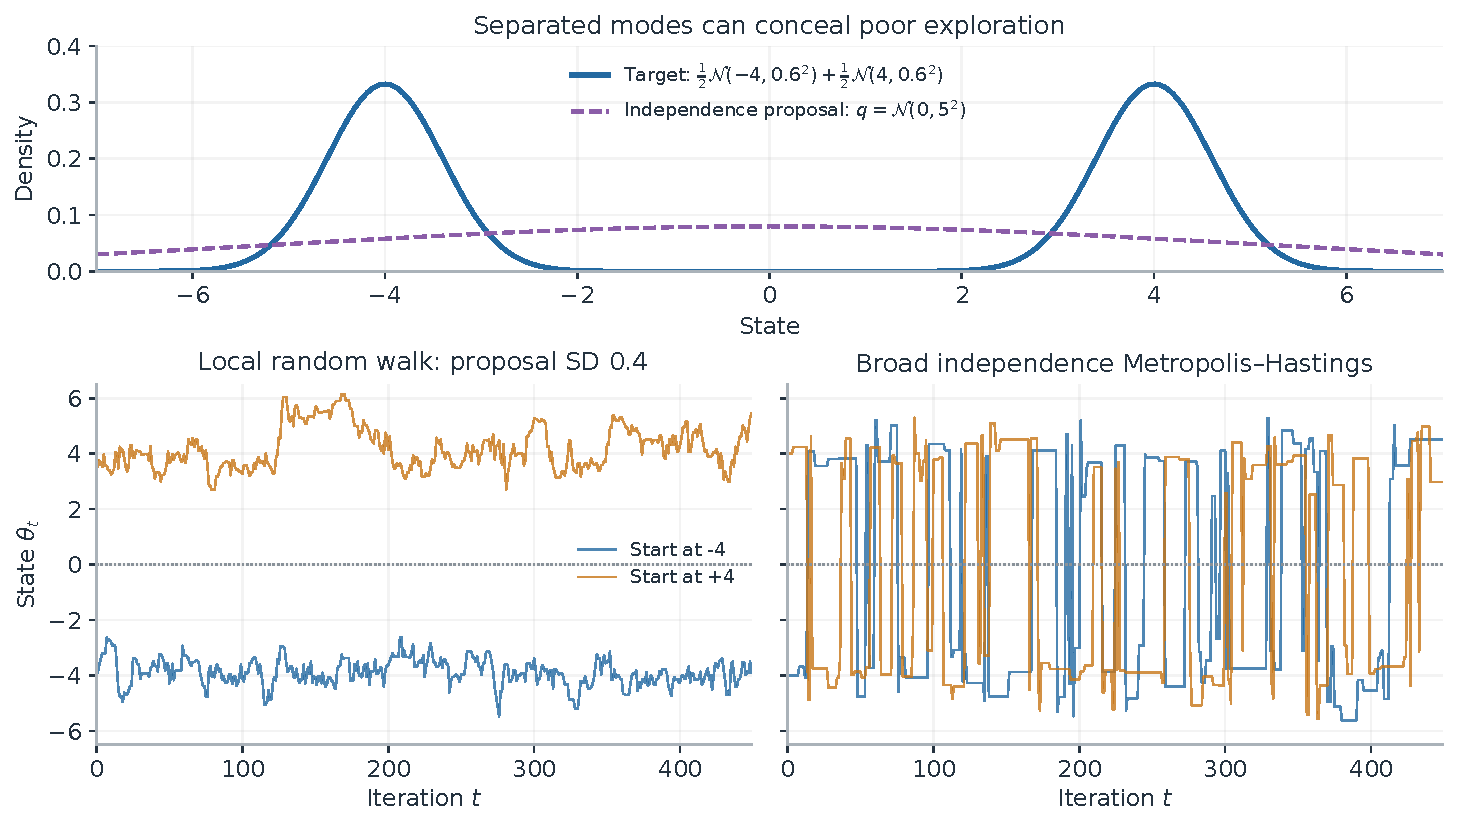
\includegraphics[width=\linewidth]{assets/multimodal_mixing.pdf}
\caption{Within-mode exploration can look satisfactory while full-mixture
exploration fails. Balanced starts can produce a plausible pooled histogram
or mean without mode exchange. A broader proposal can improve mode travel
despite accepting fewer candidates.}
\end{figure}

\subsection{The general Hastings correction}
The function takes current and candidate target log densities, then forward
and reverse proposal log densities. Its output is log acceptance, capped at zero:
\begin{lstlisting}
def mh_log_accept(lp_current, lp_candidate,
                  lq_forward, lq_reverse):
    return np.minimum(
        0.0, lp_candidate - lp_current + lq_reverse - lq_forward)
\end{lstlisting}
Forward means $q(y\mid x)$ and reverse means $q(x\mid y)$. For the
independence proposal these are $q(y)$ and $q(x)$:
\begin{lstlisting}
lq_forward = norm.logpdf(candidate, loc=0.0, scale=5.0)
lq_reverse = norm.logpdf(current, loc=0.0, scale=5.0)
log_alpha = mh_log_accept(lp_current, lp_candidate,
                          lq_forward, lq_reverse)
\end{lstlisting}
Independence from the current location does not imply conditional-proposal
symmetry. Although this proposal is symmetric around zero, generally
$q(x)\ne q(y)$. The Hastings terms do not cancel. For the Gaussian random
walk, $q(y\mid x)=q(x\mid y)$ and they do cancel.

A useful hint is to write the ratio with explicit arguments before taking
logs. A common additive constant in target log densities must cancel.
Equal proposal terms must recover the symmetric rule. Checking detailed
balance for one asymmetric pair directly verifies the orientation.

\subsection{The law obtained when the correction is omitted}
Suppose an independence sampler incorrectly uses
$\alpha_0(x,y)=\min\{1,\pi_{\rm mix}(y)/\pi_{\rm mix}(x)\}$.
Its stationary density is proportional to
\[
 \gamma(x)=\pi_{\rm mix}(x)q(x).
\]
The accepted flow under $\gamma$ is
\[
 \gamma(x)q(y)\alpha_0(x,y)
 =q(x)q(y)\min\{\pi_{\rm mix}(x),\pi_{\rm mix}(y)\},
\]
which is symmetric. Equivalently, the correct independence-MH ratio for
$\gamma$ cancels the proposal factors and becomes the incorrect target-only
ratio.

A longer run therefore reduces numerical error around the wrong distribution.
Here both $\pi_{\rm mix}$ and $q$ are symmetric around zero. Their normalized
product is symmetric too: even the wrong law has mean zero and positive-state
probability one half. Those summaries cannot detect the missing correction.
Algebraic validity and richer distributional checks are necessary.

\subsection{Mode occupancy, transitions, and model answers}
The local random walk typically explores its initial component with few or
no inter-mode transitions. Starting two chains in each mode balances the
pooled mean near zero by construction. It does not mean any individual chain
has sampled the full mixture. Each chain's positive-state fraction can remain
near zero or one, and split $\widehat R$ exposes substantial between-chain
disagreement relative to component variance.

Count sign changes between consecutive states of each retained chain and
report its positive-state fraction. These address mode exchange more directly
than acceptance alone. A smooth trace in one component shows local movement,
not global exploration. A batch MCSE calculated entirely inside one component
can be small while omitting uncertainty associated with the other.

The broad independence proposal can move directly between modes. It wastes
some candidates in low-density locations while improving global exploration.
Acceptance, mode travel, and precision per evaluation measure different
aspects of performance. No particular transition count should be required
from every realization.

The task is complete when the proposal terms have the correct orientation,
the formula reduces to the symmetric rule where appropriate, and the
interpretation separates local movement from full-mixture exploration. A
correct pooled mean from nonmixing chains is a counterexample, not a
convergence certificate.

\begin{thebibliography}{9}
\bibitem{owen}
Art B. Owen.
\emph{Monte Carlo theory, methods and examples}, Chapter 9: Importance sampling.
\href{https://artowen.su.domains/mc/Ch-var-is.pdf}{Available from the author's website}.

\bibitem{vehtari}
Aki Vehtari, Andrew Gelman, Daniel Simpson, Bob Carpenter, and Paul-Christian
B\"urkner.
Rank-normalization, folding, and localization: An improved $\widehat R$ for
assessing convergence of MCMC.
\emph{Bayesian Analysis}, 16(2):667--718, 2021.
\href{https://arxiv.org/abs/1903.08008}{arXiv:1903.08008}.
\end{thebibliography}
\end{document}
